\documentclass{beamer}
\usetheme{default}
\usepackage{float}
\usepackage{tikz}
\usetikzlibrary{positioning}

\title{Quicksort}
\author{Michele Chersich, Pratyai Mazumder, Lodovico Mazzei}
\begin{document}
\setbeamertemplate{caption}{\raggedright\insertcaption\par}
\begin{frame}[plain]
    \date{}
    \maketitle
\end{frame}
\begin{frame}{Quicksort}
    \begin{center}
        {\Large The sorting problem}
    \end{center}
\end{frame}
\begin{frame}{Sorting problems}
    \begin{center}
        \onslide<1->{Rearranging a sorted collection of elements\\}
        \onslide<2->{(usually an $n$-element array)\\}
        
        \onslide<3->{
            \begin{figure}[H]{
                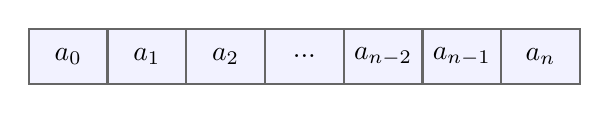
\begin{tikzpicture}[
                    squarednode/.style={rectangle, draw=black!60, fill=blue!5, thick, minimum width=10mm, minimum height=7mm, outer sep=0pt}
                ]
                    \node[squarednode] (zero) {$a_0$};
                    \node[squarednode] (one) [right=0cm of zero] {$a_1$};
                    \node[squarednode] (two) [right=0cm of one] {$a_2$};
                    \node[squarednode] (dots) [right=0cm of two] {...};
                    \node[squarednode] (nm2) [right=0cm of dots] {$a_{n-2}$};
                    \node[squarednode] (nm1) [right=0cm of nm2] {$a_{n-1}$};
                    \node[squarednode] (n) [right=0cm of nm1] {$a_n$};
                \end{tikzpicture}
            }
            \caption{Input: sequence of $n$ elements}
            \end{figure}
        }
        \onslide<4->{
            \begin{figure}[H]{
                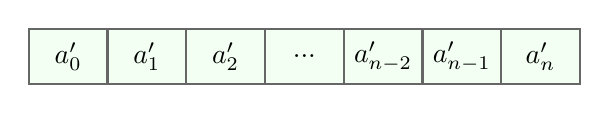
\begin{tikzpicture}[
                    squarednode/.style={rectangle, draw=black!60, fill=green!5, thick, minimum width=10mm, minimum height=7mm, outer sep=0pt}
                ]
                    \node[squarednode] (zero) {$a^\prime_0$};
                    \node[squarednode] (one) [right=0cm of zero] {$a^\prime_1$};
                    \node[squarednode] (two) [right=0cm of one] {$a^\prime_2$};
                    \node[squarednode] (dots) [right=0cm of two] {...};
                    \node[squarednode] (nm2) [right=0cm of dots] {$a^\prime_{n-2}$};
                    \node[squarednode] (nm1) [right=0cm of nm2] {$a^\prime_{n-1}$};
                    \node[squarednode] (n) [right=0cm of nm1] {$a^\prime_n$};
                \end{tikzpicture}
            }
            \caption{Output: ordered permutation}
            \end{figure}
        }
    \end{center}
\end{frame}
\begin{frame}{Worst-case runtime analysis}
    $T(n)$ is the number of comparisons, expressed by:
    \begin{align*}
        T(n) &= \max_{1\leq i\leq n-1} \{T(i)+T(n-i)\} + cn \\
        T(1) &= \Theta(1) \\
        \intertext{where $i$ is the pivot and $cn$ is partitioning time.}
        \intertext{The worst choices are $i=1$ and $i=n-1$:}
        T(n) &= \Theta(n^2)
    \end{align*}
\end{frame}
\begin{frame}{Average runtime analysis}
    Assume random input and first element pivot.
    The pivot is equally likely to be any element between 1 and n.
    \begin{align*}
        T(n) &= \frac{1}{n} \sum_{i=0}^{n-1} \left(T(i) + T(n-i)\right) + cn \\
        T(1) &= \Theta(1)
    \end{align*}
\end{frame}
\begin{frame}{Average runtime analysis}
    Assume random input and first element pivot.
    The pivot is equally likely to be any element between 1 and n.
    \begin{align*}
        T(n) &= \frac{1}{n} \sum_{i=0}^{n-1} \left(T(i) + T(n-i)\right) + cn \\
        T(n) &= \frac{2}{n} \sum_{i=0}^{n-1} T(i) + cn \\
        nT(n) &= 2 \sum_{i=0}^{n-1} T(i) + cn^2
    \end{align*}
\end{frame}
\begin{frame}{Average runtime analysis}
    Subtract the previous term of the recurrence relation:
    \begin{align*}
        nT(n) - (n-1)T(n-1) &= 2T(n-1) + 2n - c \\[1em]
        nT(n) - (n+1)T(n-1) &= 2cn \\[1em]
        \frac{T(n)}{n+1} - \frac{T(n-1)}{n} &= \frac{2c}{n+1}
    \end{align*}
\end{frame}
\begin{frame}{Average runtime analysis}
    We get the sequence of equations:
    \begin{align*}
        \frac{T(n)}{n+1} - \frac{T(n-1)}{n} &= \frac{2c}{n+1} \\
        \frac{T(n-1)}{n} - \frac{T(n-2)}{n-1} &= \frac{2c}{n} \\
        \frac{T(n-2)}{n-1} - \frac{T(n-3)}{n-2} &= \frac{2c}{n-1} \\
        \dots& \\
        \frac{T(2)}{3} - \frac{T(1)}{2} &= \frac{2c}{3}
    \end{align*}
\end{frame}
\begin{frame}{Average runtime analysis}
    Adding up all the equations:
    \begin{align*}
        \frac{T(n)}{n+1} - \frac{T(1)}{2} &= 2c\sum_{i=3}^{n+1}\frac{1}{i} \\
        \intertext{Considering the Harmonic series:}
        \sum_{i=3}^{n+1}\frac{1}{i} &= \log_e(n+1) + \gamma - \frac{3}{2} \\
        \intertext{Discarding all constant terms:}
        T(n) &= \mathcal{O}(n\log n)
    \end{align*}
\end{frame}
\end{document}
